\documentclass{scrreprt}
\usepackage{listings}
\usepackage{underscore}
\usepackage{graphicx}
\usepackage[bookmarks=true]{hyperref}
\usepackage[utf8]{inputenc}
\usepackage[english]{babel}
\usepackage[dvipsnames]{xcolor}
\setlength{\parindent}{4em}
\setlength{\parskip}{1em}
\renewcommand{\baselinestretch}{1.0}
\hypersetup{
    bookmarks=false,    % show bookmarks bar?
    pdftitle={Software Requirement Specification},    % title
    pdfauthor={Jean-Philippe Eisenbarth},                     % author
    pdfsubject={TeX and LaTeX},                        % subject of the document
    pdfkeywords={TeX, LaTeX, graphics, images}, % list of keywords
    colorlinks=true,       % false: boxed links; true: colored links
    linkcolor=blue,       % color of internal links
    citecolor=black,       % color of links to bibliography
    filecolor=magenta,        % color of file links
    urlcolor=cyan,        % color of external links
    linktoc=page            % only page is linked
}%
\def\myversion{1.0 }
\date{}
%\title
\usepackage{hyperref}
\begin{document}

\begin{flushright}
    \rule{16cm}{5pt}\vskip1cm
    \begin{bfseries}
        \Huge{PFR's MicroPortal Project\\ Documentation}\\
        \vspace{1.5cm}
        \vspace{1.5cm}
        {\LARGE Molecular \& Digital Breeding Team}\\
        \vspace{0.3cm}
        {\large New Cultivar Innovation}\\
        \vspace{1.5cm}
        \small{Version \myversion}\\
        \vspace{1.5cm}
        Prepared by : Jack Wang
        \\
        Supervisor: Amali Thrimawithana 
        
        \today\\
    \end{bfseries}
\end{flushright}

\tableofcontents

\chapter{Introduction}

\section{Objective}
One of our current projects is in establishing a pipeline for the analysis of data obtained from multiple sources (e.g. DNA and RNA sequencing, proteome) relating to a plant and its associated microbiome. Our objective is to develop a user-friendly web application to visualise the microbiome data. This could include (but not limited to) a GUI friendly front-page where the user can interact with the image of a plant through interaction the user can dive more into various microbe/microbiome information generated from data analysis relating to species/tissue. As for the back-end, user will be able to search specific project-related data, download certain files, and make comparison between different data set at different level.  In addition, integration of existing visualisation bioinformatics tools such as genome browsers/Krona/plotly/D3/Phinch/blast/interactive pathway explorer will be expected as well as the ability to search the data (Back-end).

\section{Project Scope}
The MicroPortal project was initiated by Amali Thrimawithana as part of the Discovery Science project, an initial web application prototype was developed by the students at AUT (prototype available upon request). After the prototype was established, the team saw the potential and decided to push the MicroPortal project further, to a user friendly and interactive web application product with extensive features to satisfy researcher's expectation on related projects. The team recruited Jack Wang (MInfoTech, BSc in Compsci at UoA) to finish the task.
\newline
The project started on late November, after the initial meeting on user requirement, we determined the development cycle and priorities. Overall, the project development contents were separated into front-end \& back-end. Apart of the coding process, design \& consulting with the team in advance, quality assurance \& feedback after certain feature accomplished are strictly followed during the development cycle.  
\begin{itemize}
  \item Design Principle
    \begin{itemize}
        \item Acquire necessary information and requirement from the team/researchers in advance
        \item Maximizing the user-friendliness, interactivity and intuition of the web application 
        \item Building core functions required by researchers
        \item Any additional features can be embedded into current framework seamlessly
        \item The application should be portable and accessible for future development  
    \end{itemize}
  \item Front-end 
    \begin{itemize}
        \item Establishing a home page, integrating multiple projects and their brief introduction.
        \item Diversity view page development 
        \item Comparison function for certain project
        \item About page contains project details
        \item Search result page for presenting project data, also in associate with back-end database
    \end{itemize}
  \item Back-end
  \begin{itemize}
        \item Establishing a project specified database on powerplant
        \item Apache HTTP server required (supported by powerplant) 
        \item Comparison function fetch the data from database
        \item Download function available on certain FASTA files
        \item External link/culture color labels on search result. 
    \end{itemize}
  \item QA \& Feedback
  \begin{itemize}
        \item Manual test on certain new features, fixing then re-test  
        \item Update new features to the team, waiting for feedback
        \item Collecting and analyse feedback 
        \item Fixing and improving
    \end{itemize}
\end{itemize}
 
\chapter{Installation \& User Guide} 

\section{User Instruction}
\begin{enumerate}
\item
For PFR stuff, the MicroPortal web application is available at:
\newline 
\url{https://powerplant.dev.pfr.co.nz/microPortal} 
\newline
(PFR internal network is required to access MicroPortal)
\newline
\item
For user who browse microPortal for the first time, we recommend to adjust browser's zoom in / out to suit your screen size (100\% by default).
\newline
\item
The overall web-UI should be picked up by users easily.
In the diversity view page, user can click start tour button to learn how to operate each function.
\begin{figure}[h!]
    \centering
    
\includegraphics[width=3cm,height=30pt]{Start Tour.PNG}
    \caption{Start Tour}
    \label{fig:Start Tour}
\end{figure}
\item
The search function is available to project-related data, general information is also searchable (e.g. family/genus/species etc.).If user wants more accurate result without duplicate information, either search for TaxonID/ContigID or search base on several criteria in the search combo box.     \begin{figure}[h!]
    \centering
    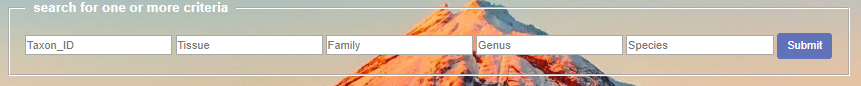
\includegraphics[width=10cm,height=30pt]{search combo box.PNG}
    \caption{Search Combo Box}
    \label{fig:Start Tour}
\end{figure}   
\end{enumerate}
\section{Developer Instruction}
\begin{enumerate}
\item For developer/PFR stuff who wants to review the source code/structure/frame of MicroPortal, the resources are available at GitHub: 
\newline
\url{https://github.com/PlantandFoodResearch/microPortal}
\newline
(Authorization may required to access the repositories)
\item Once all the files are downloaded, use source code editor (e.g. Atom, Notepad++) to browse relevant code files (.php and .html).
\newline
\item 
Front-end contents include: Home page (\textcolor{blue}{index.html}), Diversity View for two projects ( \textcolor{blue}{Discovery\_Science.html} \& \textcolor{blue}{Honey\_Landscape.html}), Contig Level Comparison for Discovery Science project (\textcolor{blue}{Comparison.html}), Culture Level Comparison for Discovery Science project (\textcolor{blue}{Culture\_Comparison.html}), About page for two projects (\textcolor{blue}{DS\_About.html} \& \textcolor{blue}{HL\_about.html}).
\item
Back-end contents are mainly focus on search function and its additional features, that include Search pages (\textcolor{blue}{Search.php} \& \textcolor{blue}{Precise\_Search.php}) and download function (\textcolor{blue}{Fasta\_download.php}).
\item 
Details about each function, framework structure and how to manipulate source code to satisfy specific project's input will be outlined in section 2.4 and 2.5.
\end{enumerate}

\section{Operating Environment}
 \begin{itemize}
 \item MicroPortal web application is able to operate in any Operating System - Mac, Windows, Linux etc. with access to browser and network.
 \item For PFR stuff, Researcher and User
 \begin{itemize}
 \item A Laptop / Desktop with access to web browsers (Chrome recommended)
 \item Have access to PFR's powerPlant server (on site or use VPN)
 \end{itemize}
 \item For developer
 \begin{itemize}
 \item Have access to PFR's powerPlant server (aklppf13)
 \item Have access to PFR's powerPlant database server (MySQL driver, DB: hraaxt\_microPortal)
 \item Have access to microPortal GitHub repository
 \item In order to develop and test efficiently, most work are required to handle locally before upload to server. Apache HTTP server is required to run php files, and connect to PFR's server locally. XAMPP control panel is recommended to install. After download, all the files can be stored under the folder path  \textcolor{blue}{XAMPP/htdocs/scripts}, type \url{http://localhost/scripts/index.html} on browser to run microPortal locally.
 \end{itemize}
 \end{itemize}


\section{Application Front-end Guide}
\begin{enumerate}
{\Large \item Homepage} (\textcolor{blue}{index.html})
\begin{itemize}
\item \begin{large}\textbf{Top Navigation Bar}\end{large}
\begin{itemize}
    \item Provide navigation to user, main features are integrated and displayed.
    \item Current version's contents:
    \begin{itemize}
        \item PFR logo
        \item MicroPortal logo
        \item Diversity View list (Discovery Science \& Honey Landscape)
        \item Blast Server quick link
        \item Comparison link (Contig Level \& Culture Level comparison)
        \item About (Discovery Science project background and details)
        \item Search Bar (Searchable on Discovery Science data)
    \begin{figure}[h!]
    \centering
    
\includegraphics[width=15cm,height=30pt]{Navbar.PNG}
    \caption{Top Navigation Bar}
    \label{fig:Start Tour}
\end{figure}
    \end{itemize}
    \item For developer to alter/manipulate navigation contents, simply change the code between 
      \textcolor{blue}{$<$header$>$} and \textcolor{blue}{$<$/header$>$} in each file.
     \item The CSS \& JavaScript code that define certain style and feature can be traced by class name in the same code sheet.
     \newline
\end{itemize}

\item 
\begin{large}\textbf{Welcome to MicroPortal}\end{large}
\begin{itemize}
    \item Welcome slogan with modern style design, font type and size are picked for sending simple, friendly message, as well as draw user's attention by using the large font size.
    \begin{figure}[h!]
    \centering
    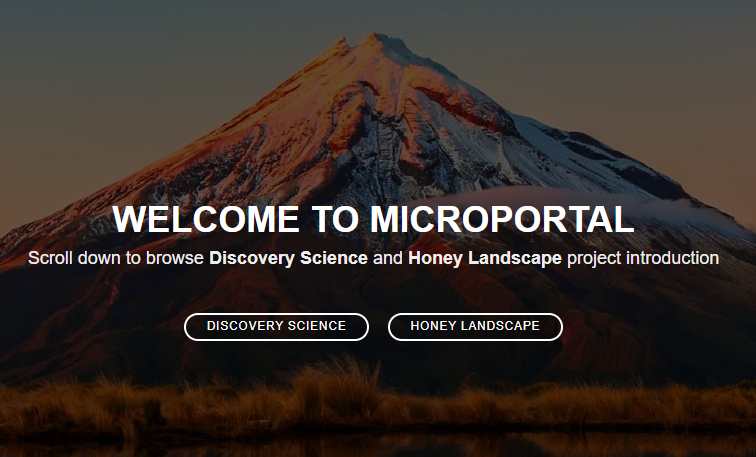
\includegraphics[width=10cm,height=6cm]{Welcome.PNG}
    \caption{Welcome to MicroPortal}
    \label{fig:Start Tour}
\end{figure} 
    \item Quick links for browsing DS and HL projects' diversity view page.
    \item Instruction for user to scroll down to browse more information, also the top of following section displayed on the main page to show user that there are more contents available on the same page.
    \item The iconic Mount Taranaki is selected as background. Change of the background is allowed for specific project in future development.
    \item For developer to alter/manipulate the contents in welcome section, simply trace the class: \textcolor{blue}{$<$section id="hero"$>$} in each file.
\end{itemize}
\item 
\begin{large}
\textbf{Project Brief Introduction}
\end{large}
\begin{itemize}
    \item Project's logo is placed on the right side with description on the left
    \item Diversity view link is available, more links that relate to the project can be added. 
    \item For developer to alter/manipulate the contents in introduction section, simply trace the classes for two projects: \textcolor{blue}{$<$section id="about" class="DiscoverySci"$>$} and \textcolor{blue}{$<$section id="about" style="" class="honeyland"$>$}.
\end{itemize}
\end{itemize}
{\Large \item Diversity View} (\textcolor{blue}{Discovery\_Science.html} \& \textcolor{blue}{Honey\_Landscape.html})
\begin{itemize}
    \item \begin{large}\textbf{Discovery Science }\end{large}(\textcolor{blue}{Discovery\_Science.html})
    \begin{itemize}
        \item \textbf{DS: Mānuka Microbiome button}
        \newline
        Project title, user can click the button, then browse DS project details. For manipulating/altering the contents, this section starts from \textcolor{blue}{$<$div class="header" id="rcorners1"$>$}.
    \begin{figure}[h!]
    \centering
    
\includegraphics[width=5cm,height=1cm]{DSbutton.PNG}
    \caption{Portal to Project Details}
    \label{fig:Start Tour}
\end{figure}
    \item \textbf{Tour button}
    \newline
    User can click "Start Tour", then follow the instruction to explore each function on DS diversity view page. Source code in html: \textcolor{blue}{$<$input type="button" class="btn btn-lg" id="rcorners2" onclick="startTour()" value="Start Tour" /$>$}, JavaScript function: \textcolor{VioletRed}{function} \textcolor{blue}{startTour()}. 
    \begin{figure}[h!]
    \centering
    
\includegraphics[width=3cm,height=1cm]{Start Tour.PNG}
    \caption{Diversity View Tour}
    \label{fig:Start Tour}
\end{figure}
\item \textbf{Left Side Navigation}. 
\newline 
This panel contains basic instruction, plant tissue outline and project location/specie details. The side navigation bar provides additional information/features to user, it is both easy to use (simply mouse hover on the icon) and extensible (more options/icons can be added to existing navigation bar for different projects). 
\begin{figure}[h!]
    \centering
    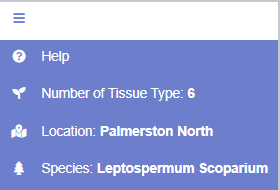
\includegraphics[width=6cm,height=4cm]{Side Nav Bar.PNG}
    \caption{Side Navigation}
    \label{fig:Start Tour}
\end{figure}
\newline
For developer to manipulate/change the contents in navigation bar, tracing the following class name: \textcolor{blue}{$<$div class = "left"$>$}
\newline
\item \textbf{Interactive Plant Image}. 
\newline 
As the main function in the diversity view page, user can explore Discovery Science project data by interacting with this plant image. This plant image is in .svg format, we've added many interactive elements and established multi-layer structure for user to explore each tissue's visualized data.
\newline
\begin{figure}[h!]
    \centering
    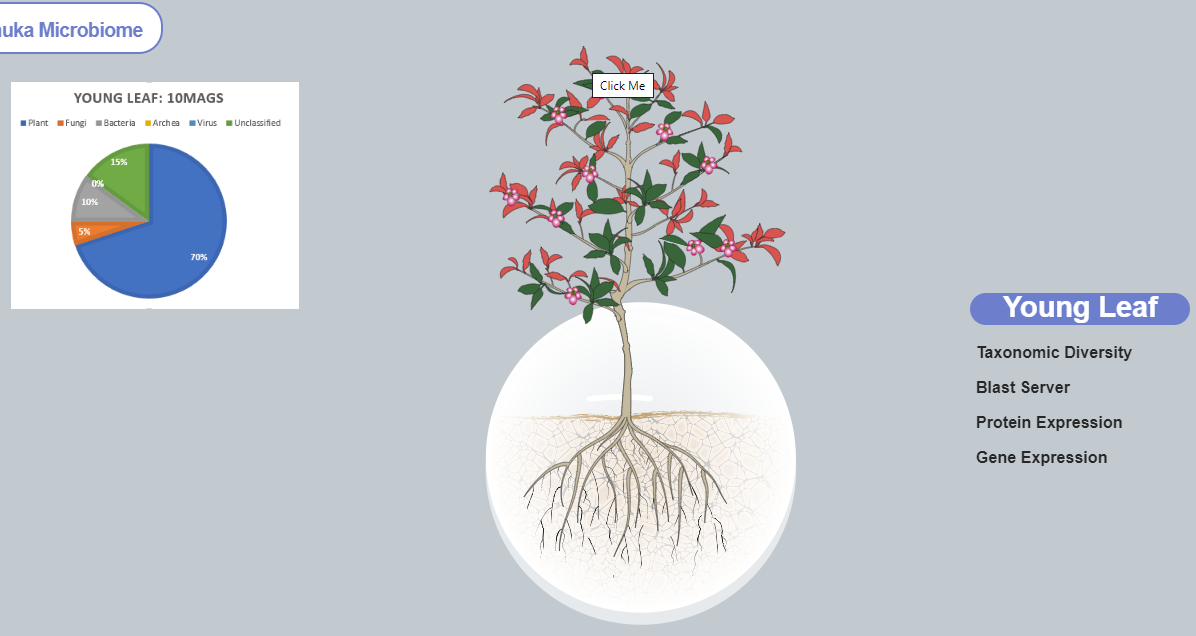
\includegraphics[width=12.5cm,height=7cm]{Plant.PNG}
    \caption{Interactive Plant}
    \label{fig:Start Tour}
\end{figure}
\newline
For developer to manipulate/alter the content/style/multi-layer structure, they should have previous knowledge about SVG path property and its relevance to CSS and JavaScript. The section includes plant svg and preview pie chart starts from  \textcolor{blue}{$<$div class="plant-section" id="plant"$>$}, the right-side panel appears after click each tissue starts from \textcolor{blue}{$<$div class="side-categories" id="NAV1"$>$} to \textcolor{blue}{$<$div class="side-categories" align="left" id="NAV6"$>$} for six tissues. 
\newline
\item \textbf{Biocultural Metadata Panel}. 
\newline
The panel appears on the right side contains Discovery Science project's biocultural metadata.
\newline
\begin{figure}[h!]
    \centering
    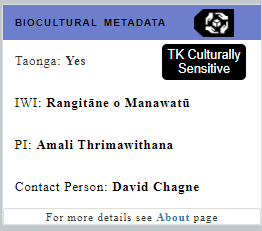
\includegraphics[width=5cm,height=4cm]{BioMetadata.PNG}
    \caption{Biocultural Metadata}
    \label{fig:Start Tour}
\end{figure}
User can learn if the plant is a Taonga specie, the type of traditional knowledge label (in this case, it is culturally sensitive), the IWI of this plant and the details of initiative person/contact person.

For developer to add/change the current contents, the code starts with class name: \textcolor{blue}{$<$div class="wrapper center-block"$>$}
\end{itemize}
    \item \begin{large}\textbf{Honey Landscape }\end{large}(\textcolor{blue}{Honey\_Landscape.html})
    \begin{itemize}
        \item \textbf{Honey\_Landscape button on the top-left}
        \newline
        Project title, similar as the button introduced in Discovery Science section. User can click to enter the project detailed background page. The code for this part starts with class name: \textcolor{blue}{$<$div class="header" id="rcorners1"$>$}
    \begin{figure}[h!]
    \centering
    
\includegraphics[width=5cm,height=1.2cm]{HLtitle.PNG}
    \caption{Honey Landscape Project Title}
    \label{fig:Start Tour}
\end{figure}
        \item \textbf{Side Navigation Bar}
        \newline
        The left side navigation bar, which contains general information relates to the project. Developer can add extra icon/contents base on different projects. This panel starts with class name: \textcolor{blue}{$<$div class="left"$>$}
         \begin{figure}[h!]
    \centering
    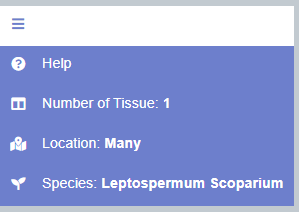
\includegraphics[width=5.5cm,height=3.5cm]{HLsidenav.PNG}
    \caption{Honey Landscape Project Title}
    \label{fig:Start Tour}
\end{figure}
        \item \textbf{Interactive NZ Map}
       \newline
       For Honey Landscape project, the data are located in five regions of New Zealand: 
       \begin{itemize}
           \item Auckland
           \item Bay of Plenty
           \item Manawatu-Wanganui
           \item Otago
           \item Southland
       \end{itemize}
       \begin{figure}[h!]
    \centering
    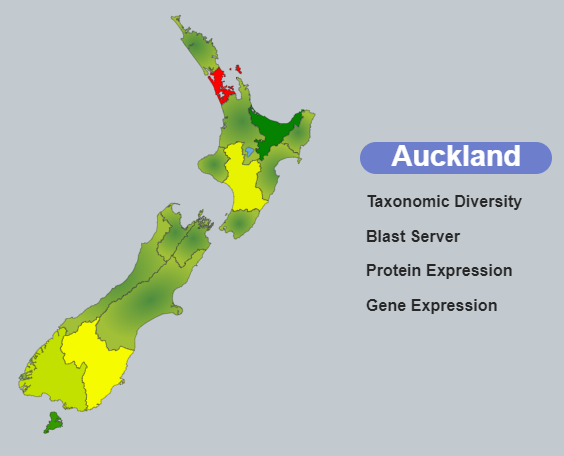
\includegraphics[width=7.5cm,height=5cm]{HLAuckland.PNG}
    \caption{Interactive NZ map}
    \label{fig:Start Tour}
\end{figure}
       Each region has been highlighted with color transition effect, that shows which region's data is available to user.
       Same as DS project's interactive plant section, user can click each region to browse various data expression visualisation.
       \newline
       Developer can alter the interactive map svg contents and change the operation mode. The map section starts with the class: \textcolor{blue}{ $<$div class="NZ\_map\_new"$>$}, all the relevant CSS/JS code can be traced by class name within the section. 
        \item \textbf{Biocultural Metadata Panel}
        \newline
        Features are same as Discovery Science's metadata panel with different contents. Developer can add/remove contents, alter interact method/style, the panel starts with the class:
        \newline
        \textcolor{blue}{$<$div id="collapseOne" class="panel-collapse collapse in sub_panel" 
        \newline 
        role="tabpanel" aria-labelledby="headingOne"$>$}
        \begin{figure}[h!]
    \centering
    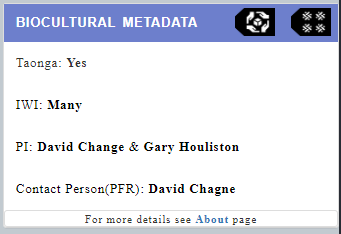
\includegraphics[width=7.5cm,height=5cm]{HLBM.PNG}
    \caption{Honey Landscape Biocultural Metadata}
    \label{fig:Start Tour}
\end{figure}
\newline
\newline
        \item \textbf{Tour Button}
        \newline
        Same operation mode as introduced in previous section. 
    \end{itemize}
\end{itemize}

{\Large \item Comparison} (\textcolor{blue}{Comparison.html} \& \textcolor{blue}{Culture_Comparison.html})
\newline
\newline
MicroPortal can not only display project information and microbe data visualisation, but also offers customized project data comparison at different levels. The comparison function for Discovery Science project is implemented, and we want this function to be more flexible, portable and extensible, as we intend to integrate the comparison function into future projects. The following two pages are Discovery Science Comparison Guide at metagenomic - contig level and culture level. 
\begin{itemize}
\item \begin{large}\textbf{Metagenomic - Contig Level Comparison }\end{large}(\textcolor{blue}{Comparison.html})
\begin{itemize}
    \item \textbf{Anychart.js}
    \newline
    All the comparison Venn diagrams and pie charts are generated using Anychart.js (trial version), it is a open source chart generation tool without license requirement. For details, please visit:
    \newline
    \url{https://www.anychart.com/}
    \item \textbf{Data Input}
    \newline
    Most diagram/charts are automatically generated using the data from Powerplant db server where all the project related data are stored. 
    Due to the limitation of Anychart.js, some of the input data were manually imported for the purpose of accuracy. For the future development, we are seeking ways to fully automate the process with high accuracy (data crawling algorithm combine with scalable chart generation tools, pipeline etc.)
    \newline
    \item \textbf{User Guide}
    \newline
    For both metagenomic - contig level \& culture comparisons, user can compare up to three tissue type with selective compare type. As the Venn diagram displayed on the right side, user can see the tissue name with amount of value under it. User can mouse hover on each Venn diagram section to browse Species/Genus/Family/Culture information, then click each section to view the data proportion pie chart which contains amount and percent value.
    \begin{figure}[h!]
    \centering
    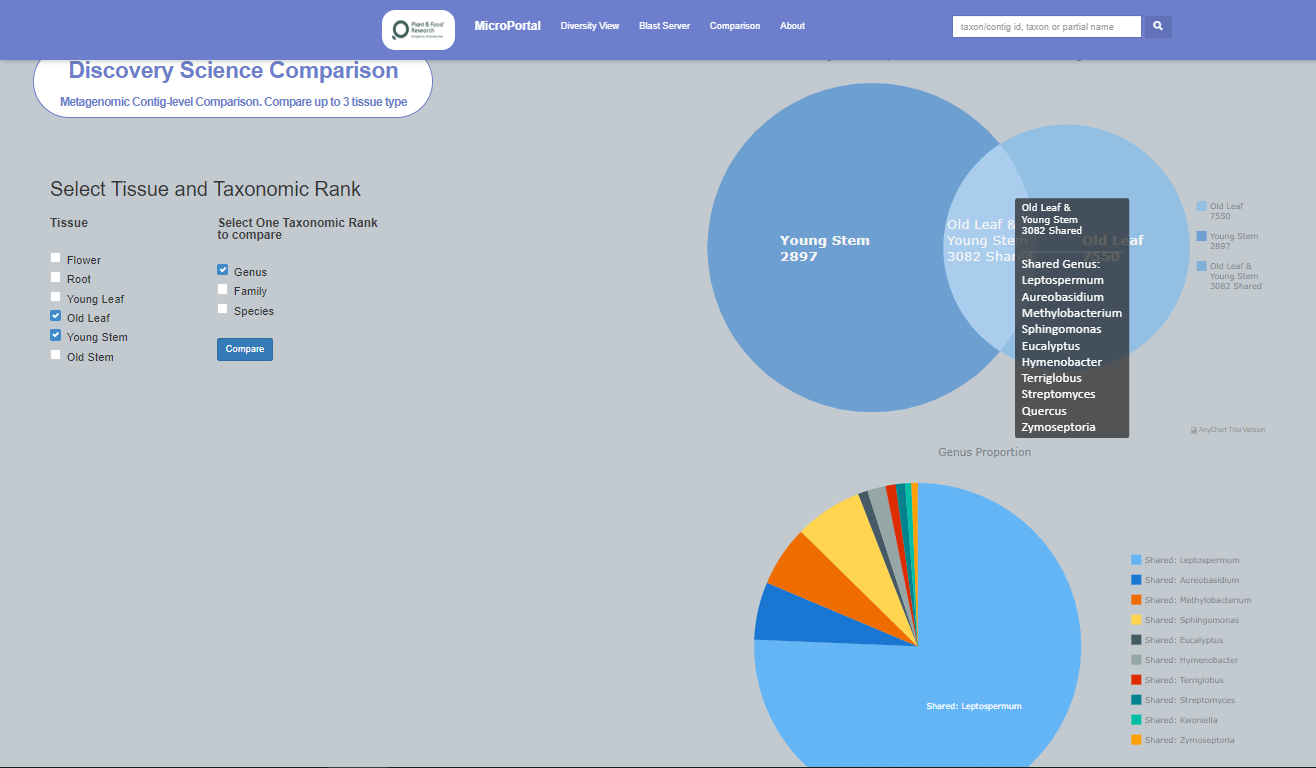
\includegraphics[width=13cm,height=7.5cm]{Comparison.PNG}
    \caption{Metagenomic Comparison}
    \label{fig:Start Tour}
\end{figure}
\end{itemize}
\item \begin{large}\textbf{Culture Level Comparison }\end{large}(\textcolor{blue}{Culture Comparison.html})
\newline
\newline
Culture comparison has the same functionality as metagenomic comparison, it uses culture data to compare each tissue. 
\end{itemize}
   

\end{enumerate}

\section{Application Back-end Guide}
\begin{enumerate}
\item {\Large Database}
\newline
\newline
We deployed our database on Powerplant Database Server:
\newline
\url{https://powerplant.pfr.co.nz/dbaas/}
\newline For Discovery Science project, we set up a database to store all the project-related data. The structure we use is relational database MySQL. In the future, we might switch to NoSQL DBMSs for its light weight structure, quick access to massive datasets.
\newline
For developer to access the database, they will be required to have authorization on DB username: \textcolor{blue}{hraaxt\_microbiom}, the database name is \textcolor{blue}{hraaxt\_microPortal} and the table name:  \textcolor{blue}{DS_Data}. More information is available in the code file   \textcolor{blue}{Search.php}.
\item {\Large Powerplant Server}
\newline
\newline
In order to establish MicroPortal access for all PFR stuff in a portable and easy way, we deployed the web application on Powerplant development server \textcolor{blue}{aklppf13}, under the directory:  \textcolor{blue}{/var/www/html/microPortal}, all the web application updates should go through this route.  
\item {\Large Search Page} (\textcolor{blue}{Search.php} \& \textcolor{blue}{Precise_Search.php})
\newline
\newline
The search engine is powered by .php and MySQL database. User can search for any key word in the project datasets. In the case of Discovery Science, the main searchable terms include taxon/contig ID, taxonomy name for species, genus and family. The average time for searching is between 2-3 seconds. The search bar is placed on the top-right of Discovery Science Diversity View page, and other DS related pages (comparison etc.). Note that this database is specific established for DS project, and the data is not applied on other projects (Honey Landscape etc.). 
\newline
\newline
Due to the massive datasets and large amount of duplicated information (only contig ids are unique), we set up a precise search function to let user searches up to five criteria, in order to display user's expected search results.
\begin{figure}[h!]
    \centering
    
\includegraphics[width=15cm,height=1.5cm]{PreciseSearch.PNG}
    \caption{Precise Search Function}
    \label{fig:Start Tour}
\end{figure}
\newline
The search page is also include download function, user can simply click the Contig ID to download the corresponding FASTA file.
\begin{figure}[h!]
    \centering
    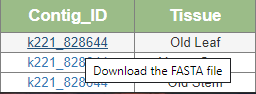
\includegraphics[width=5cm,height=2cm]{FastaDownload.PNG}
    \caption{FASTA Download}
    \label{fig:Start Tour}
\end{figure}
\begin{figure}[h!]
    \centering
    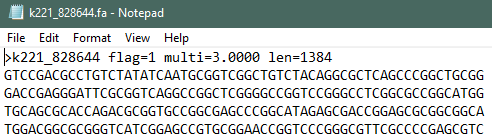
\includegraphics[width=10cm,height=3cm]{FastaFile.PNG}
    \caption{FASTA file}
    \label{fig:Start Tour}
\end{figure}
\newline
\newline
\newline
In addition, for scientific purpose, we colorized the genus type under three conditions: genomic support, culturing support, and both genomic \& culturing support. The colors are outlined as white, yellow and green.
\begin{figure}[h!]
    \centering
    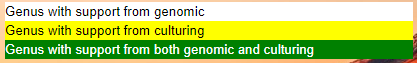
\includegraphics[width=8cm,height=1.5cm]{ColorGenus.PNG}
    \caption{Colorized Genus}
    \label{fig:Start Tour}
\end{figure}
\newline
In the search results, user can identify the category of genus by its background color. As the screen capture shows below, the same genus under different tissues would have different support from genomic/culturing.
\begin{figure}[h!]
    \centering
    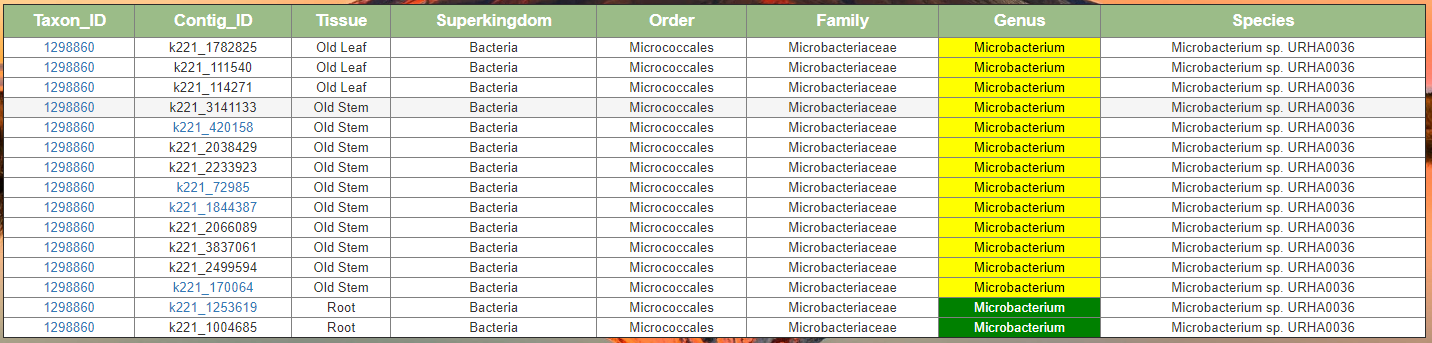
\includegraphics[width=15cm,height=4.5cm]{GenusTable.PNG}
    \caption{Search Table Demo}
    \label{fig:Start Tour}
\end{figure}
\end{enumerate}

\chapter{Summary \& Future Development}
During the first four months development period, the MicroPortal framework has been successfully established as a functional product and microbe data visualisation tool. Currently, two projects: Discovery Science \& Honey Landscape had been integrated in the framework. And with the deployment on Powerplant server, PFR stuffs can take a look and provide valuable feedback.

For the future development and maintenance, we plan to bring more PFR projects into this framework, the projects will not limited to microbe or specific types. And we will provide more functions to satisfy scientific requirements. We will have discussion with the scientists who showed interests and happy to display their project data on the web application. For start, the original home page had been modified to be able to fit more projects in a user friendly way, and we are open to any feedback and suggestion. Feel free to contact Jack Wang (\href{mailto:Jack.Wang@plantandfood.co.nz}{Jack.Wang@plantandfood.co.nz}) and Amali Thrimawithana (\href{Amali.Thrimawithana@plantandfood.co.nz}{Amali.Thrimawithana@plantandfood.co.nz}) for any questions.  
\newline


\end{document}